\chapter{Resultados Experimentais}\label{cap:results}

\section{Aquisição de dados}

Para os experimentos realizados neste trabalho foi capturado um conjunto de vídeos no estacionamento do pavilhão João Calmon na Universidade de Brasília. Foram feitas duas seções de filmagens contínua, aonde três veículos se deslocavam pelo estacionamento e ocupavam vagas escolhidas arbitrariamente. O primeiro vídeo capturado foi utilizado para o treinamento da rede. O segundo vídeo foi dividido em oito vídeos de menor duração sobre os quais foram realizados os testes.

As filmagens foram realizadas por um drone modelo ????\ref{fig:???}. O drone foi controlado para que pairasse no ar em uma altura semelhante a de um poste de luz, a fim de capturar imagens de forma mais próxima possível de uma câmera de vídeo instalada em um poste de luz.

%Descobrir o modelo do drone e colocar uma imagem%

Para a aquisição das imagens utilizadas para o treinamento da rede, o primeiro vídeo passou por um processo semelhante ao processo de calibração do programa final descrito no capítulo \ref{cap:solucao}. Duas áreas de interesse foram determinadas de forma idêntica ao processo de escolha de ROIs do programa. Em seguida cada ROI foi dividida em trinta seções verticais. Três quadros do vídeo foram escolhidos de forma aleatória. As imagens correspondentes a cada seção de cada quadro escolhido foram extraídas em arquivos separados. Dessa maneira, as imagens utilizadas para o treinamento da rede neural foram construídas da mesma maneira que as imagens que seriam alimentadas a ela para classificação no futuro.

\section{Treinamento da rede neural artificial}

Uma vez adquiridas as imagens a serem utilizadas para o treinamento, cada uma delas foi separada manualmente em uma das duas categorias:veículo ou vaga vazia. Ao todo foram utilizadas $57$ imagens classificadas como veículo(categoria 1) e $59$ imagens classificadas como vaga vazia(categoria 2) totalizando $116$ imagens. Foram extraídas as características de cada imagem da forma descrita na seção \ref{sec:extracao}. Os vetores $x_s$ obtidos foram então concatenados de forma a criar duas matrizes. A primeira de dimensões $6x57$ representava as \textit{features} das imagens de carros e a segunda de dimensões $6x59$ as características das imagens de vagas desocupadas.

\begin{figure}
\centering
\begin{subfigure}{.1\textwidth}
  \centering
  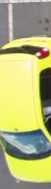
\includegraphics[width=.8\linewidth, height=5cm]{ocupada}
  \caption{}
  \label{fig:exemploRede:sub:ocupada}
\end{subfigure}%
\begin{subfigure}{.1\textwidth}
  \centering
  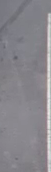
\includegraphics[width=.8\linewidth, height=5cm]{desocupada}
  \caption{}
  \label{fig:exemploRede:sub:desocupada}
\end{subfigure}
\centering
\caption{(a)Um exemplo de imagem classificada manualmente na classe 1.(b) Um exemplo de imagem classificada manualmente na classe 2.}
\end{figure}

Para que pudesse ser feito o treinamento supervisionado da rede neural, duas matrizes de alvos foram construídas. Uma com dimensões $2x57$ e a outra com dimensões $2x59$. A primeira matriz com todas as colunas iguais a $\begin{psmallmatrix}1\\0\end{psmallmatrix}$ e a segunda com as colunas da forma $\begin{psmallmatrix}0\\1\end{psmallmatrix}$. Essas matrizes vão compor o gabarito utilizado para o treinamento supervisionado da rede.

As matrizes  de características de cada classe foram então concatenadas formando uma matriz de entrada $In_{6x116}$. O mesmo foi feito com as matrizes do gabarito, resultando na matriz $Target_{2x116}$. Em seguida as colunas dessas duas matrizes foram reorganizadas aleatoriamente, de forma que as mudanças feitas em $In$ fossem refletidas em $Out$, garantindo que não fosse perdida a relação entre as colunas de mesmo índice das matrizes. O resultado final deste processo é que cada coluna de $Target_{2x116}$ indica a classe da coluna correspondente de $In_{6x116}$.

Uma vez criadas essas duas matrizes, as entradas e seus respectivos alvos são separados em três conjuntos: o conjunto de treinamento, de validação e de testes. A divisão é feita de forma que $70\%$ das entradas são designadas ao conjunto de treinamento, $15\%$ designadas ao conjunto de validação e os $15\%$ restantes ao conjunto de testes. O conjunto de treinamento então é composto por duas matriz $Ti_{6x81}$ e $To_{2x81}$ que são iguais as primeira $81$ colunas de $In_{6x116}$ e $Target_{2x116}$ e representam os vetores descritores das entradas e seus gabaritos respectivamente. Os outros dois conjuntos são construídos de forma similar utilizando. O conjunto de validação é composto por matrizes de $18$ colunas e o de teste por matrizes de $17$ colunas.


A rede neural utilizada foi uma rede \textit{feed-forward} com três camadas. A camada oculta possui $15$ neurônios com função de ativação logística (\ref{eq:logistica}) e a camada de saída $2$ neurônios com função de ativação \textit{softmax} (\ref{eq:softmax}). A rede é submetida a um treinamento supervisionado com um limite de $1000$ iterações. Quando a situação de convergência é atingida, o treinamento para e o resultado é a rede final utilizada.




















